\documentclass{article}

\usepackage{graphicx}
\usepackage[legalpaper, portrait, margin=1in]{geometry}
\usepackage{xcolor}
\usepackage{color,soul}
\newcommand\todo[1]{\textcolor{red}{#1}}

\usepackage{subcaption}


\title{Supervised Learning - CS7641 Fall 2021}
\author{Huifu Tian}
\begin{document}
\maketitle


In this assignment, I will use the Polish companies bankruptcy data set and the MNIST handwritten digits data set to compare various supervised learning algorithms. All of the analysis was done using the scikit-learn library compatible with Python 3.



\section{Polish Data}

\subsection{Data Overview}
This dataset is a collection of Polish companies spanning 2007-2013. The dataset contains a total of roughly 700 bankrupt companies corresponding to 2400 financial reports in the period between 2007 and 2013. The data is separated into five datasets - 1stYear, 2ndYear, 3rdYear, 4thYear, 5thYear. Each row in every data set contains the financial report of one company in a single year. \newline

- 1stYear: 7027 surveyed companies in 2007, 271 of which went bankrupt by the start of 2013

- 2ndYear: 10173 surveyed companies in 2008, 400 of which went bankrupt by the start of 2013

- 3rdYear: 10503 surveyed companies in 2009, 495 of which went bankrupt by the start of 2013

- 4thYear: 9792 surveyed companies in 2010, 515 of which went bankrupt by the start of 2013

- 5thYear: 5910 surveyed companies in 2011, 410 of which went bankrupt by the start of 2013\newline


The attributes are shown in Appendix Table 1. \newline

The output consists of one column where 1 means bankruptcy and 0 means non-bankruptcy. \newline

\todo{add more stats exploring the data such as autocorrelations, class sizes, etc}


\subsection{Preprocessing}

Minimal preprocessing was done to keep the focus on analysis. I combined all of the data sets to form a new dataset of over 43000 rows, which may introduce oversampling bias since it's not guaranteed that each company that is marked with a bankruptcy status=1 only shows up once across the 5 data sets. \todo{is it called oversampling bias?} All of the infrequent NaNs in the attribute columns are replaced with 0's. (There are no NaNs in the output column.) I divide the data into 70\% train and 30\% test sets while applying stratification to ensure uniform distribution of classes between the two groups. Finally, I under sample the majority class to a 1:1 ratio when evaluation the performance of a model and when I apply StratifiedKFolds to create validation scores. This is done to address the issue of a 95:5 imbalanced dataset and that most of the algorithms evaluated in this study is biased towards fitting to the majority class samples.


\subsection{Decision Tree}

\subsubsection*{Baseline model}

The baseline model uses sklearn's DecisionTreeClassifier class and is trained with unlimited tree depth and the Gini measure of impurity. Table 2 shows the mean metric scores from fitting the classifier on the training data and scoring on the test data. With undersampling, I mean the results across 20 iterations of random sampling from the majority class before doing the fitting.


\begin{table}
	\centering
	Table 1: Baseline Model Performance
	\begin{tabular}{ l l l l l l | l l l l l }
		\hline
		              &DT  & NN & KNN& XGB & SVM & DT & NN & KNN & XGB & SVM \\
		             \hline
		Undersampling?&No  &No  &No  & No &No  &Yes &Yes &Yes &Yes &Yes \\
		Accuracy      &0.95&0.94&0.95&0.97&0.95&0.78&0.57&0.65&0.86&0.65\\
		F1            &0.48&0.01&0.02&0.63&0.00&0.78&0.57&0.65&0.87&0.63\\
		Precision     &0.46&0.11&0.10&0.89&0.50&0.78&0.58&0.65&0.86&0.68\\
		Recall        &0.50&0.03&0.01&0.49&0.00&0.79&0.58&0.65&0.88&0.59\\

		\hline 
		
		
	\end{tabular}
	\footnotetext[1]{Only one iteration of fitting}
	\footnotetext[2]{ratio of the post-undersampled majority to minority class}
\end{table}



\begin{figure}
	\centering
	Figure 1: Decision Tree Validation Curves\\
	\begin{subfigure}{.24\textwidth}
		a: Max Depth
		\centering
		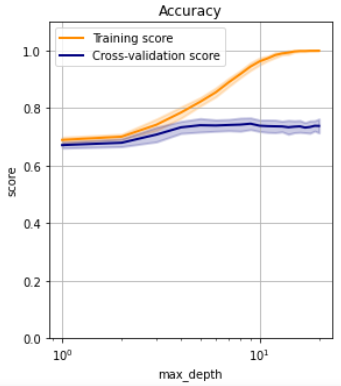
\includegraphics[width=\linewidth]{poland_decision_max_tree_depth_accuracy.png}
		
	\end{subfigure}%
	\begin{subfigure}{.24\textwidth}
		b: Min Samples Split
		\centering
		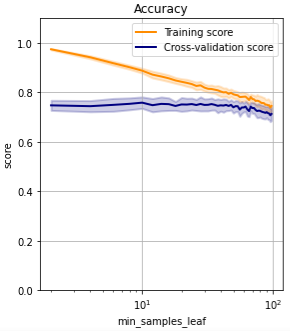
\includegraphics[width=\linewidth]{poland_decision_min_samples_split_accuracy.png}
		
	\end{subfigure}
	\begin{subfigure}{.24\textwidth}
		c: Min Samples Leaf
		\centering
		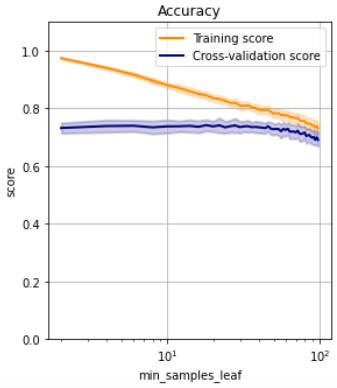
\includegraphics[width=\linewidth]{poland_decision_min_samples_leaf_accuracy.png}
		
	\end{subfigure}
	\begin{subfigure}{.24\textwidth}
		d: Min Impurity Decrease
	\centering
	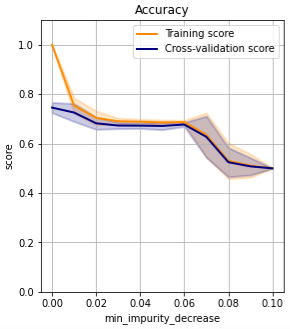
\includegraphics[width=\linewidth]{poland_decision_min_impurity_decrease_accuracy.png}
	
	\end{subfigure}

	\label{fig:test}
\end{figure}


Before tuning the model, it's worth noting that the decision tree classifier exhibits the general behavior one tends to see with imbalanced data sets, namely that the classifier prefers to minimize error for the majority class at the expense of the minority class. As the sample rebalancing approaches parity between both classes (shown by the progression from 3:1 to 1:1 ratio), precision, recall, and accuracy of the minority class are all improved. As a bonus, fitted tree depth also becomes smaller, which is preferred because we like simpler models over more complex models. \newline

\subsubsection*{Model Tuning}
\subsubsection*{Impurity}
I first experiment with using "Gini" or "entropy" as the impurity measure. I find that there's no significant difference in any of the accuracy/f1/precision/recall scores using the undersampled data. Since the entropy measure takes longer to calculate due to logs in the measure and it doesn't offer significant improvements, I use "Gini" for the rest of the analysis.


\subsubsection*{Max Tree Depth}
\todo{ try fit to max depth and use pruning}
Without bounding max tree depth, the baseline model will fit the data to a tree with average depth of 19.65 using 1:1 rebalancing across 20 random samplings across the majority class. I also use a modified version of the Stratified K Folds validation algorithm. Rather than selecting k folds to split one set of the post-undersampled training data into a train and validation set, I select 2 folds across k sets of training data. The reason for this modification is that I'm undersampling the majority class. To reduce the variance of results across multiple trials as much as possible, hence k folds, it makes more sense to randomly pick from a much bigger pool of data than to undersample first then pick from a smaller pool of data. 
Figure 1a shows the accuracy score of modulating the max\_depth from 1 to 20. The training curve is generally increasing while the cross validation curve increases and tapers off. The reason is increasing the max tree depth allows the model to fit the training data to increasing accuracy. With a tree of around 20 nodes deep, the model is able to almost perfectly fit the training data. For the cross validation score, the highest score is reached at max\_depth=9 (see Table 2). At that point, the accuracy scores starts to decrease and overfitting occurs. 

\subsubsection*{Min Samples Split}
Min samples split is a pruning threshold that requires each node to have at least a certain number of samples before it's split again. I range this parameter from 2 to 500 while letting max tree depth to be unlimited. The performance of the model is reported in Table 2 col 2 and the validation curve is shown in Figure 1b. The training curve starts at 100\% accuracy and gradually decreases. this is because at value of 1 corresponds to no pruning and the decision tree can perfectly predict the training set. The accuracy score on the validation set is flat up until 100 and slows drops down. The flatness of this curve from 2 to 100 indicates there is a collection of nodes that are split just with fewer than 100 samples. The further splitting of that collection of nodes offer no additional benefit to the model once that node has been established. What we can learn from analyzing this parameter is that our data is very noisy and a few high-level splits determine our model's predictive behavior. 

\subsubsection*{Min Samples Leaf}
The validation curves are shown in Figure 1c. The training and validation curves are both very similar to those of min samples split. We attempt to increase this parameter to reduce the variance and limit overfitting. But we learn that increasing this parameter only hurts the model's ability to generalize. We only start losing prediction power once we remove nodes that have 15+ samples, which means that all the nodes that are smaller than 15 samples are a coin flip and the model's architecture cannot handle further complexity. 

\subsubsection*{Min Impurity Decrease}

\todo{ this section}

\begin{center}
	Table 2: Decision Tree Parameter Tuning Results
	\begin{tabular}{ l l l l l }
		\hline
		Metric & Max Tree Depth & Min Samples Split & Min Samples Leaf & haha \\
		\hline
		Accuracy & 0.79 & 0.77 & 0.81 & 0.79 \\
		F1 & 0.79 & 0.77 & 0.71 & 0.79 \\
		Precision & 0.78 & 0.77 & 0.71 & 0.78 \\
		Recall & 0.79 & 0.77 & 0.72 & 0.79 \\
		Optimal Value & 9 & $<=$100 & $<=$15 & 19.75\\
		\hline 
		
		
	\end{tabular}
\end{center}


\subsection*{Learning Curves}

To understand whether our model is overfitting or underfitting, I make two learning curves: one without restrictions, one with max tree depth. In the case without setting max\_depth, the training accuracy scores stay at roughly 100\%. This shows that the model was likely too complex and fit the training model perfectly. The idea that this model is overfitting the data is also supported by the fact that the validation scores remain flat, meaning that the model is unable to generalize. Once I introduce max\_depth, the training model's accuracy scores start to decrease as we limit the model's complexity. The result is that a simpler model does better at generalization, which is shown by the much improved scores on the test data. There is still a gap between the training curve and the validation curve at the 2000th sample, which means that further limiting of the model's complexity may improve the validation score. Also, validation scores are still in the middle of improving at the 2000th sample, which implies that having more samples would improve the model's ability to fit the data. \todo{discuss variance and bias}

\begin{figure}
\centering
Figure 2
\begin{subfigure}{.5\textwidth}
\centering
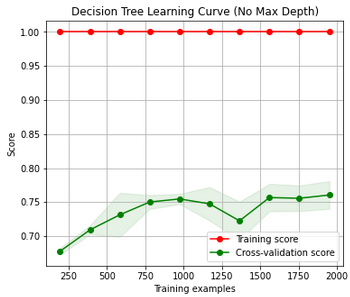
\includegraphics[width=\linewidth]{poland_decision_learning_curve_without_max_depth.png}

\end{subfigure}%
\begin{subfigure}{.5\textwidth}
\centering
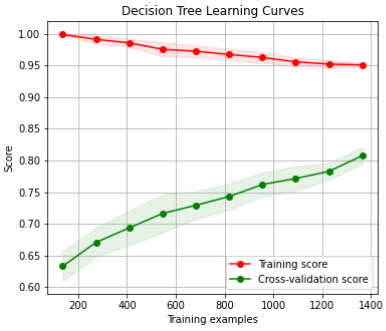
\includegraphics[width=\linewidth]{poland_decision_learning_curve_with_max_depth.png}

\end{subfigure}
\label{fig:test}
\end{figure}

\subsubsection*{Final model and performance}

The model with max\_depth set to 9 yields is run 20 times using 1:1 balanced sampling between the two classes, each time picking a 70\% training and 30\% testing set. The mean accuracy across the 20 iterations is 0.79. \todo{Show in final summary table}

\subsection{Neural Network}

\subsubsection*{Baseline model}

The baseline results with and without undersampling the majority class are shown in Table 1. The rest of the analysis will undersample the majority class. The parameters default to using a single hidden layer with 30 nodes and 1e-4 as regularization alpha. I also scale the features to have mean 0 and variance 1. 


\begin{figure}
	\centering
	Figure 3: Neural Network\\
	\begin{subfigure}{.3\textwidth}
		\centering
		3a: Hidden Layer 1 \# Nodes
		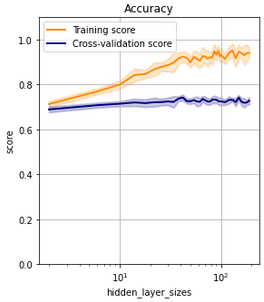
\includegraphics[width=\linewidth]{poland_nn_hidden_layer_size_2_200_accuracy.png}
		
	\end{subfigure}
	\begin{subfigure}{.3\textwidth}
		\centering
		3b: Hidden Layer 2 \# Nodes
		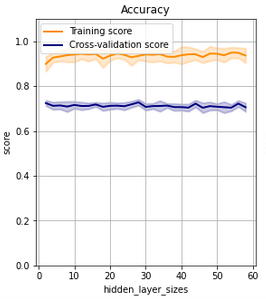
\includegraphics[width=\linewidth]{poland_nn_hidden_layer_2_size_2_60_accuracy.png}
		
	\end{subfigure}
	\begin{subfigure}{.3\textwidth}
		\centering
		3c: Regularization Alpha\\
		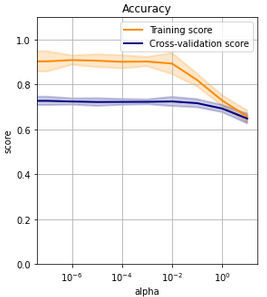
\includegraphics[width=\linewidth]{poland_nn_alpha_0_10_accuracy.png}
		
	\end{subfigure}
	\label{fig:test}
\end{figure}

\subsubsection*{Model Tuning}

\subsubsection*{Size of Hidden Layers}
The training and cross validation accuracy scores by varying the number of nodes in a one-hidden layer net are shown in Figure 3.The accuracy curve on the train set starts low but increases as more complexity is enabled on the model. Also at first, the increasing complexity in the model benefits the validation scores. The question is what's the optimal number of nodes in the hidden layer that maximizes generalization accuracy? And the answer is 42. Any further increases in model complexity only marginally increases the model fit on the training data while gradually lowering the ability to generalize on the validation set. This is overfitting. One can also see from the training scores after n=42 start to display higher variance, which means that the model's accuracy becomes more dependent on particular idiosyncrasies in the weights and the data itself. \todo{check last sentence.}

At this point, I can do a grid search to find the optimal number of nodes on a 2-hidden layer network. But before that, I will hold the number of nodes at 42 on the first layer and repeat the same procedure as before on the second layer. The results are shown in Figure 4. As you can see, the accuracy on the cross-validation curve is flat, which shows that the extra layer does not seem to add further benefits to the 1-layer model. 

\subsubsection*{Regularization Alpha}

Another parameter to vary is the L2 regularization alpha. This parameter is the multiplicative scalar term of a penalty term added to the cost function. The penalty term is the sum of the weights squared multiplied by alpha/2, which means that any model that minimizes this function will also need to make sure the weights are small as well. The larger the alpha, the greater the penalty and more we can limit potential overfitting. The results are presented in Figure 5 and Table 5 Column 6. The training and test curves in Figure 5 show that there's no difference in adjusting alpha between 0 and 1e-2. After 1e-2, higher alphas starts to limit the model's complexity and leads to underfitting. This is observed by the decreasing testing score metric. The various metric scores in column 6 show no difference using 1e-7 as the alpha value. 


\begin{table}

	\centering
	Table 3: Neural Network Parameters and Results\\
	\begin{tabular}{ l l l }
		\hline
		Parameter & Hidden Layer 1 Size& alpha\\
		\hline
		Accuracy & 0.75 & 0.75 \\
		F1 & 0.75 & 0.74 \\
		Precision & 0.75 & 0.75 \\
		Recall & 0.76 & 0.74\\
		Optimal Value & 42 & $<=$1e-2 \\

	
		\hline 
	\end{tabular}
\end{table}

\subsection*{Learning Curves}



\subsection{KNN}
\subsubsection*{Baseline Model}

The baseline model results with and without undersampling are shown in Table 1. Like decision trees and neural nets, KNN is susceptible to showing partiality to the majority class. Also like neural nets, the features need to be normalized to mean 0 and variance 1. This is because the distance measure used to determine the set of k nearest neighbors will place more weight on features that have the larger scale. For example, the model cares a lot about features that are big because larger features result in larger distances. In reality, there is no reason aside from having domain knowledge to weigh one feature more than another. 


\subsubsection*{Model Tuning}
\subsubsection*{Number of Neighbors K}

The validation curves on from varying the number of k nearest neighbors are shown in Figure 6. The training scores on all of the score metrics generally start high and decreases as the number of neighbors increase. This is expected because having fewer neighbors means that at least one of the fewer neighbors can vote in favor of itself. For example, in the case that k=1, picking a query sample q from the training set and and evaluating it against every data point means that the closest data point is itself and the distance is 0. In this case the accuracy on the entire training set will be 100\%. Conversely, having k=1 means that the validation set will only have one opinion from one closest neighbor, leading to noise in accuracy and hence underfitting. Increasing k reduces the effect of noise from the k nearest neighbors and improves the accuracy. However, continuing to increase k to the size of the training set means that every vote will result in the majority class winning. The result is an accuracy score that's identical to the proportion of majority class in the dataset. And the model becomes useless. The validation curves for f1, precision, and recall show some instability of when k$<$10. This is the result of the way sklearn resolves ties among even numbers of neighbors. The algorithm returns the lowest class value which is always 0. The effect of this behavior has a particularly strong effect on recall, since the number of false negatives is usually high when votes are always broken to create additional false negatives. Column 5 shows the performance of the model while selecting the k that optimizes the validation score. In our case, the same max value was reached at k=11 and k=52, so I simply average these values and round down to the lower odd value. (I could round up as well)


\begin{figure}
	\centering
	Figure 4:\\
	\begin{subfigure}{.26\textwidth}
		\centering
		4a: Validation curve of k
		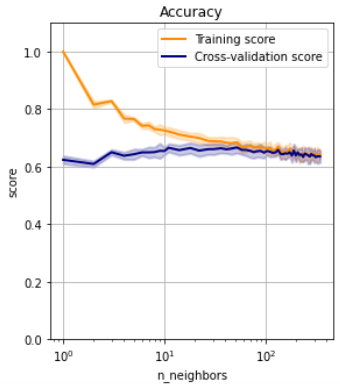
\includegraphics[width=\linewidth]{poland_knn_n_neighbors_350_accuracy.png}
		
	\end{subfigure}
	\begin{subfigure}{.34\textwidth}
		\centering
		4b: Learning Curve, k=31
		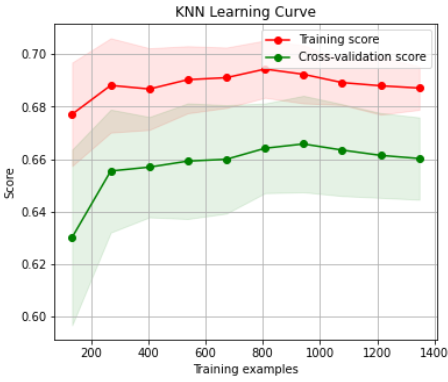
\includegraphics[width=\linewidth]{poland_knn_learning_curve.png}
	
	\end{subfigure}
	\begin{subfigure}{.35\textwidth}
	\centering
		3c: Learning Curve, k=5
	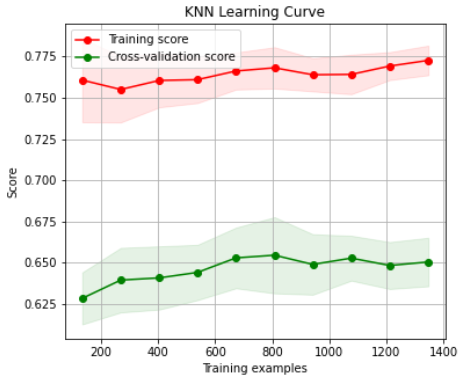
\includegraphics[width=\linewidth]{poland_knn_learning_curve_k_5.png}
	
\end{subfigure}

	\label{fig:test}
\end{figure}


\begin{table}
	
	\centering
	Table 4: KNN Parameters and Results\\
	\begin{tabular}{ l l l l l l l }
		\hline
		Parameter & 1 & 2 & 3 & 4 & 5 & 6\\
		\hline
		n\_neighbors & 5 & 5 & 5 & 5 & \hl{31} & 31 \\
		weights & uniform & uniform & uniform & uniform & uniform & \hl{distance} \\
		algorithm & auto & auto & auto & auto & auto & auto \\
		p & 2 & 2 & 2 & 2 & 2 & 2\\
		Undersampled? & No & \hl{3:1} & \hl{1:1} & 1:1 & 1:1 & 1:1 \\
		Normalized? & No & No & No & \hl{Yes} & Yes & Yes\\
		\hline
		Results & & & & & \\
		\hline
		Accuracy & 0.95 & 0.74 & 0.65 & 0.66 & 0.67 & 0.67\\
		F1 & 0.02 & 0.38 & 0.65 &  0.66 & 0.66 & 0.65\\
		Precision & 0.10 & 0.47 & 0.65 & 0.66 & 0.69 & 0.69\\
		Recall & 0.01 & 0.31 & 0.65 &  0.65 & 0.63 & 0.63\\
		Balanced accuracy & 0.50 & 0.60 & 0.65 & 0.66 & 0.67 & 0.67\\
		
		\hline 
	\end{tabular}
\end{table}


\subsection*{Learning Curves}

The learning curve for KNN is shown in Figure 7. Both curves are fairly flat with the exception of the smallest sample size. It's also possible to argue that the curves increase slightly before peaking around 800-1000 samples before tapering off again, though the difference is only from 68\% to 69\% for the training set. If this increase can be argued, the explaination would be that adding more samples only improves accuracy for both the training and testing sets only up to a certain point before too many data points are added. If the data is noisy, or if irrelevant features are used in the distance calculations, the algorithm would actually be incapable of learning from the dataset. In our case, it looks like adding more data would not help KNN learn better. We would probably need to explore the features and weigh them differently to address autocorrelations, irrelevant features, etc. 


\subsection{Boosting}
\subsubsection*{Baseline Model}
I fit the data using XGBoost, following the same process as the before on undersampling, improving f1, precision, recall, and balanced accuracy. \todo{ alternative ways to handle this? } The baseline results are shown in Table 1. The parameters used for the results are as follows: n\_estimators=100, max\_depth=10. No pruning was performed. Note that we don't have to normalize data because the decision tree weak classifier only needs absolute feature values to work. 

\subsubsection*{Model Tuning}
\subsubsection*{n estimators}
I adjust the number of base estimators used (n\_estimators) and plot accuracy scores on the training set as well as the validation set. The results are shown in Figure 8. Both training and validation scores start low and gradually increase as more estimators are added. Using one estimator essentially means trying to model the data with one decision tree. As more trees are added, the fit on the training and validation sets get better. The point at which 100\% of the training data is predicted perfectly also corresponds to when we start to overfit on the validation data. The model performance is shown in Table 5 column 3. 


\begin{figure}
	\centering
	Figure 5:\\
	\begin{subfigure}{.19\textwidth}
		\centering
		a: n estimators\\
		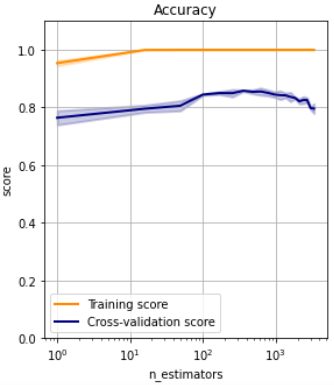
\includegraphics[width=\linewidth]{poland_xgb_n_estimators_accuracy.png}
		
	\end{subfigure}
	\begin{subfigure}{.19\textwidth}
		\centering
		b: max depth\\
		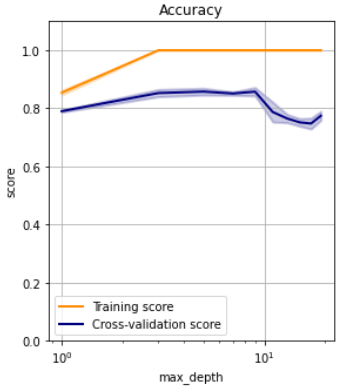
\includegraphics[width=\linewidth]{poland_xgb_max_depth_accuracy.png}
		
	\end{subfigure}
	\begin{subfigure}{.19\textwidth}
		\centering
		c: min samples split\\
		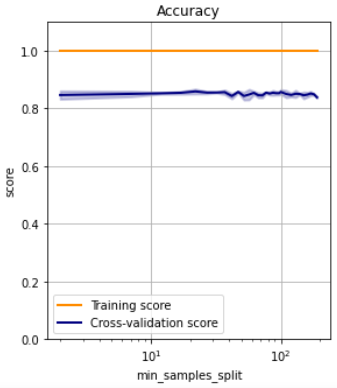
\includegraphics[width=\linewidth]{poland_xgb_min_samples_split_accuracy.png}
		
	\end{subfigure}
	\begin{subfigure}{.19\textwidth}
		\centering
		d: min samples leaf\\
		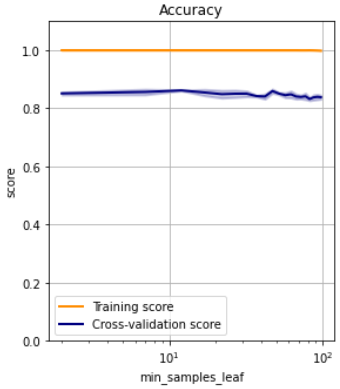
\includegraphics[width=\linewidth]{poland_xgb_min_samples_leaf_accuracy.png}
		
	\end{subfigure}
	\begin{subfigure}{.19\textwidth}
		\centering
		e: min impurity dec\\
		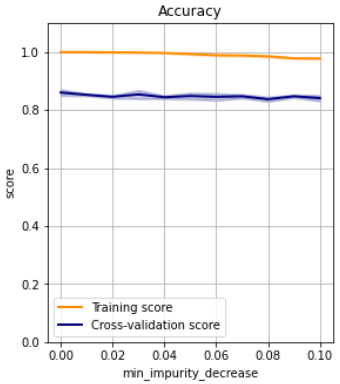
\includegraphics[width=\linewidth]{poland_xgb_min_impurity_decrease_accuracy.png}
		
	\end{subfigure}

	\label{fig:test}
\end{figure}


\subsubsection*{Max Tree Depth}
The validation curve for modulating the prepruning parameter max\_depth is in figure 5b. The optimal value of 9 is the value of max\_depth when the accuracy score on the cross-validation curve is at its highest point. In Figure 5b, accuracy scores increase for both training and validation sets but drops off for validation set after max\_depth reaches 9. This is because we are initially giving our model the complexity that is needed to fit the validation and training sets better. Too much complexity occurs after max\_depth=9 and validation scores decrease. The model performance is shown in table 5, and we can see that pre-pruning improves model performance slightly. 

\subsubsection*{Min Samples Split/Leaf}
In Figure 5c, I modulate min\_samples\_split while letting the tree to grow without max depth. n\_estimators is set to the optimal value from the previous step. Both accuracy curves are flat, which means that most of the model's predictive ability comes from the number of estimators, and not how complex any of the estimators are in terms of min\_samples\_split. Figure 5d shows the performance on the train/validation sets by pruning using the min\_samples\_leaf parameter and letting each tree grow fully. Both curves are flat, indicating no benefit to pruning using this parameter having determined the optimal number of estimators

\subsubsection*{Min Impurity Decrease}
Figure 5e shows the train/validation curves from modulating min impurity decrease, \todo{explain this and expand section}

\begin{table}
	
	\centering
	Table 5: XGBoost Results \\
	\begin{tabular}{ l c c c c c c }
		\hline
		& base & n estimators & max depth & min samples & min samples & min impurity\\
		& model & & & split & leaf & decrease \\
		\hline
		Accuracy & 0.86 & 0.87 & 0.89 & 0.87 && \\
		F1 & 0.87 & 0.87 & 0.89 & 0.87 & &\\
		Precision & 0.86 & 0.88 & 0.89 & 0.87 && \\
		Recall & 0.88 & 0.86 & 0.90 & 0.87 && \\
		Optimal value & None & 625 & 9 & 20 & & \\

		
		\hline 
	\end{tabular}
\end{table}

\subsection*{Learning Curve}
\begin{figure}
	\centering
	Figure 6:\\
	\begin{subfigure}{0.4\textwidth}
		\centering
		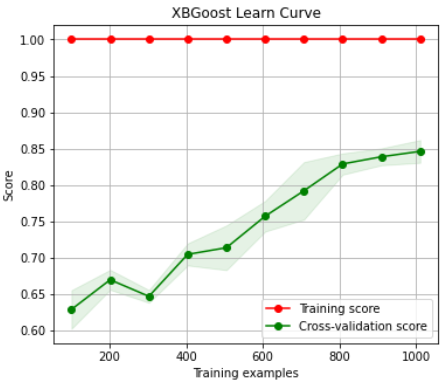
\includegraphics[width=\linewidth]{poland_xgb_learning_curve.png}
		
	\end{subfigure}
	
	\label{fig:test}
\end{figure}

\subsection{SVM}
\subsubsection*{Baseline Model}
The results from a baseline fit using rbf kernel with and without undersampling are shown in table 1. 

\subsubsection*{Model Tuning}
\subsubsection*{Kernel}
The baseline results from experimenting with ``linear'', ``polynomial'', ``rbf'', and ``sigmoid'' kernels are shown in Table 6 and Figure 7. It can be seen that the the ``linear'' and ``rbf'' kernels seem to do the best in terms of accuracy and ``polynomial'' does poorly in f1 and recall. 

\begin{figure}
	\centering
	Figure 7: Kernel\\
	\begin{subfigure}{\textwidth}
		\centering
		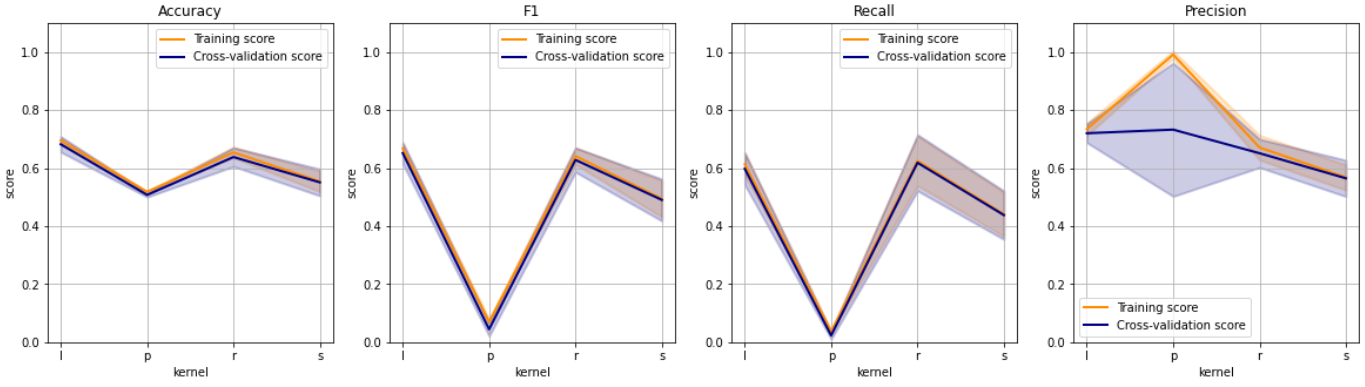
\includegraphics[width=\linewidth]{poland_svm_kernel.png}
		
	\end{subfigure}
	
	\label{fig:test}
\end{figure}

\subsubsection*{Tuning RBF}
\subsubsection*{C Regularization Parameter}


\begin{table}
	
	\centering
	Table 6: SVM Results \\
	\begin{tabular}{ l c c c c }
		\hline
		& linear & poly & rbf & sigmoid\\
		\hline
		Accuracy & 0.68 & 0.51 & 0.64 & 0.51 \\
		F1 & 0.66 & 0.05 & 0.64 & 0.41 \\
		Precision & 0.72 & 0.63 & 0.64 & 0.51  \\
		Recall & 0.60 & 0.03 & 0.66 & 0.35 \\
		\hline 
	\end{tabular}
\end{table}

\section{MNIST Data}
\subsection{Data Overview}
The MNIST data set contains 70,000 samples of 28x28 pixel handwritten digits from 0 to 9. Unlike the Polist bankruptcy data set, there are more than 10 times more number of features and 10 output classes instead of 2. The predictive knowledge in the MNIST data is more distributed among a larger set of features whereas the knowledge in the bankruptcy data is more concentrated among a smaller set of features. This can lead to the models having very different performance metrics between these two datasets. 

\subsection{Preprocessing}
I load the MNIST data through Keras and load them into the standard train/test sets where 60,000 samples are in the train set and 10,000 samples are in the test set. To see the effectiveness of parameter tuning and relative predictive abilities of the various models, I only consider the first 10,000 samples from the training set, which will be further divided into 50\% train and 50\% validation sets used during parameter tuning. Finally, I one-hot encode the output vector which contains 10 possible values ranging from 0 to 9. This is usually done on categorical outputs but I include the results from both scenarios in table 7. 

\begin{table}
	\centering
	Table 1: Baseline Model Performance
	\begin{tabular}{ l l l l l l | l l l l l }
		\hline
		&DT  & NN & KNN& XGB & SVM & DT & NN & KNN & XGB & SVM \\
		\hline
		One-hot encoding?&No  &No  &No  & No &No &Yes &Yes &Yes &Yes &Yes \\
		Accuracy      &0.81&0.94&0.95&0.97&   &0.81&0.57&0.65&0.86&  \\
		\hline 
		
		
	\end{tabular}
	\footnotetext[1]{Only one iteration of fitting}
	\footnotetext[2]{ratio of the post-undersampled majority to minority class}
\end{table}

 
\subsection{Decision Tree}


\begin{center}
	Appendix Table 1: Polish companies bankruptcy data attributes
	\centering
	\begin{tabular}{| l | l |}
		\hline
		X1 net profit / total assets                                                                                                                                       & {X33 operating expenses / short-term liabilities}                                                                                      \\ \hline
		X2 total liabilities / total assets                                                                                                                                & {X34 operating expenses / total liabilities}                                                                                           \\ \hline
		X3 working capital / total assets                                                                                                                                  & X35 profit on sales / total assets                                                                                                           \\ \hline
		X4 current assets / short-term liabilities                                                                                                                         & X36 total sales / total assets                                                                                                               \\ \hline
		\begin{tabular}[c]{@{}l@{}}X5 [(cash + short-term securities + receivables \\- short-term liabilities) \\/ (operating expenses - depreciation)] * 365\end{tabular} & X37 (current assets - inventories) / long-term liabilities                                                                                   \\ \hline
		X6 retained earnings / total assets                                                                                                                                & X38 constant capital / total assets                                                                                                          \\ \hline
		X7 EBIT / total assets                                                                                                                                             & X39 profit on sales / sales                                                                                                                  \\ \hline
		X8 book value of equity / total liabilities                                                                                                                        & \begin{tabular}[c]{@{}l@{}}X40 (current assets - inventory - receivables) \\/ short-term liabilities\end{tabular}                            
		\\ \hline
		X9 sales / total assets                                                                                                                                            & \begin{tabular}[c]{@{}l@{}}X41 total liabilities \\/ ((profit on operating activities + depreciation) \\$\times$ (12/365))\end{tabular}               
		\\ \hline
		X10 equity / total assets                                                                                                                                          & X42 profit on operating activities / sales                                                                                                   \\ \hline
		\begin{tabular}[c]{@{}l@{}}X11 (gross profit + extraordinary items \\+ financial expenses) \\/ total assets\end{tabular}                                           & X43 rotation receivables + inventory turnover in days                                                                                        \\ \hline
		X12 gross profit / short-term liabilities                                                                                                                          & X44 (receivables * 365) / sales                                                                                                              \\ \hline
		X13 (gross profit + depreciation) / sales                                                                                                                          & X45 net profit / inventory                                                                                                                   \\ \hline
		X14 (gross profit + interest) / total assets                                                                                                                       & X46 (current assets - inventory) / short-term liabilities                                                                                    \\ \hline
		\begin{tabular}[c]{@{}l@{}}X15 (total liabilities * 365) 
			\\	/ (gross profit + depreciation)         \end{tabular}                        
		& X47 (inventory * 365) / cost of products sold                                                                                                \\ \hline
		X16 (gross profit + depreciation) / total liabilities                                                                                                              & \begin{tabular}[c]{@{}l@{}}X48 EBITDA / total assets\end{tabular}                          
		\\ \hline
		X17 total assets / total liabilities                                                                                                                               & \begin{tabular}[c]{@{}l@{}}X49 EBITDA / sales\end{tabular}                                 
		\\ \hline
		X18 gross profit / total assets                                                                                                                                    & X50 current assets / total liabilities                                                                                                       \\ \hline
		X19 gross profit / sales                                                                                                                                           & X51 short-term liabilities / total assets                                                                                                    \\ \hline
		X20 (inventory * 365) / sales                                                                                                                                      & X52 (short-term liabilities * 365) / cost of products sold)                                                                                  \\
		X21 sales (n) / sales (n-1)                                                                                                                                        & X53 equity / fixed assets                                                                                                                    \\ \hline
		X22 profit on operating activities / total assets                                                                                                                  & X54 constant capital / fixed assets                                                                                                          \\ \hline
		{X23 net profit / sales}                                                                                                                                     & X55 working capital                                                                                                                          \\ \hline
		X24 gross profit (in 3 years) / total assets                                                                                                                       & X56 (sales - cost of products sold) / sales                                                                                                  \\ \hline
		X25 (equity - share capital) / total assets                                                                                                                        & \begin{tabular}[c]{@{}l@{}}X57 (current assets - inventory - short-term liabilities) \\/ (sales - gross profit - depreciation)\end{tabular}  
		\\ \hline
		X26 (net profit + depreciation) / total liabilities                                                                                                                & X58 total costs /total sales                                                                                                                 \\ \hline
		\begin{tabular}[c]{@{}l@{}}X27 profit on operating activities \\/ financial expenses \end{tabular}
		& X59 long-term liabilities / equity                                                                                                           \\ \hline
		X28 working capital / fixed assets                                                                                                                                 & X60 sales / inventory                                                                                                                        \\ \hline
		X29 logarithm of total assets                                                                                                                                      & X61 sales / receivables                                                                                                                      \\ \hline
		X30 (total liabilities - cash) / sales                                                                                                                             & X62 (short-term liabilities *365) / sales                                                                                                    \\ \hline
		X31 (gross profit + interest) / sales                                                                                                                              & X63 sales / short-term liabilities                                                                                                           \\ \hline
		X32 (current liabilities * 365) / cost of products sold                                                                                                            & X64 sales / fixed assets
		\\
		\hline                                                                                                    
	\end{tabular}
\end{center}

\end{document}